\documentclass[a4paper,12pt]{article}
%%%%%%%%%%%%%%%%%%%%%%%%%%%%%%%%%%%%%%%%%%%%%%%%%%%%%%%%%%%%%%%%%%%%%%%%%%%%%%%%%%%%%%%%%%%%%%%%%%%%%%%%%%%%%%%%%%%%%%%%%%%%%%%%%%%%%%%%%%%%%%%%%%%%%%%%%%%%%%%%%%%%%%%%%%%%%%%%%%%%%%%%%%%%%%%%%%%%%%%%%%%%%%%%%%%%%%%%%%%%%%%%%%%%%%%%%%%%%%%%%%%%%%%%%%%%
\usepackage{eurosym}
\usepackage{vmargin}
\usepackage{amsmath}
\usepackage{graphics}
\usepackage{epsfig}
\usepackage{framed}
\usepackage{subfigure}
\usepackage{fancyhdr}

\setcounter{MaxMatrixCols}{10}
%TCIDATA{OutputFilter=LATEX.DLL}
%TCIDATA{Version=5.00.0.2570}
%TCIDATA{<META NAME="SaveForMode"CONTENT="1">}
%TCIDATA{LastRevised=Wednesday, February 23, 201113:24:34}
%TCIDATA{<META NAME="GraphicsSave" CONTENT="32">}
%TCIDATA{Language=American English}

\pagestyle{fancy}
\setmarginsrb{20mm}{0mm}{20mm}{25mm}{12mm}{11mm}{0mm}{11mm}
\lhead{MA4128} \rhead{Kevin O'Brien} \chead{Week 9} %\input{tcilatex}

%http://www.electronics.dit.ie/staff/ysemenova/Opto2/CO_IntroLab.pdf
\begin{document}

\tableofcontents
\newpage
%R Classes : Machine Learning and Neural Networks
\subsection*{What is Logistic Regression?}
Logistic regression is a discriminitive probabilistic classification model that operates over real-valued vector inputs. 

The dimensions of the input vectors being classified are called "features" and there is no restriction against them being correlated. 

Logistic regression is one of the best probabilistic classifiers, measured in both log loss and first-best classification accuracy across a number of tasks.

Logistic regression requires extensive tuning in the form of feature selection and implementation to achieve state-of-the-art classification performance.

\section{Logistic Regression}
Logistic regression determines the impact of multiple independent variables
presented simultaneously to predict membership of one or other of the two
dependent variable categories.

\subsection{The purpose of logistic regression}
The crucial limitation of linear regression is that it cannot deal with Dependent Variables’s that are \textbf{\textit{dichotomous}} and categorical. Many interesting variables in the business world are dichotomous: for
example, consumers make a decision to buy or not buy (\textit{\textbf{Buy/Don't Buy}}), a product may pass or fail quality control (\textit{\textbf{Pass/Fail}}), there are good or poor credit risks (\textit{\textbf{Good/Poor}}), an employee may be promoted or not (\textit{\textbf{Promote/Don't Promote}}).


A range of regression techniques have been developed for analysing data with categorical dependent
variables, including logistic regression and discriminant analysis (Hence referred to as DA, which is the next section of course).

Logistical regression is regularly used rather than discriminant analysis when there are only two categories
for the dependent variable. Logistic regression is also easier to use with SPSS than DA when
there is a mixture of numerical and categorical Independent Variables’s, because it includes procedures for
generating the necessary dummy variables automatically, requires fewer assumptions, and
is more statistically robust. DA strictly requires the continuous independent variables  (though dummy variables can be used as in multiple regression). Thus, in instances where
the independent variables are categorical, or a mix of continuous and categorical, and the
DV is categorical, logistic regression is necessary.

\subsection{Use of Binomial Probability Theory}
Since the dependent variable is dichotomous we cannot predict a numerical value for it
using logistic regression, so the usual regression least squares deviations criteria for best fit
approach of minimizing error around the line of best fit is inappropriate.

Instead, logistic regression employs binomial probability theory in which there are only two values to
predict: that probability (p) is 1 rather than 0, i.e. the event/person belongs to one group
rather than the other. Logistic regression forms a best fitting equation or function using the
maximum likelihood method (not part of course), which maximizes the probability of classifying the observed
data into the appropriate category given the regression coefficients.

\subsection{Variable Selection}
Like ordinary regression, logistic regression provides a coefficient \textbf{b} estimates, which measures
each IV’s partial contribution to variations in the response variables. The goal is to correctly predict
the category of outcome for individual cases using the most parsimonious model.

To accomplish this goal, a model (i.e. an equation) is created that includes all predictor variables that are useful in predicting the response variable. Variables can, if necessary, be entered into the model in the order specified by the researcher in a stepwise fashion like regression.

There are two main uses of logistic regression:
\begin{itemize}
\item The first is the prediction of group membership. Since logistic regression calculates the
probability of success over the probability of failure, the results of the analysis are in
the form of an \textbf{odds ratio}.
\item Logistic regression also provides knowledge of the relationships and strengths among
the variables (e.g. playing golf with the boss puts you at a higher probability for job
promotion than undertaking five hours unpaid overtime each week).
\end{itemize}

\subsection{Assumptions of logistic regression}
\begin{itemize}
\item Logistic regression does not assume a linear relationship between the dependent and
independent variables.
\item The dependent variable must be a dichotomy (2 categories).
(Remark: Dichotomous refers to two outcomes. Multichotomous refers to more than two outcomes).
\item The independent variables need not be interval, nor normally distributed, nor linearly
related, nor of equal variance within each group.
\item The categories (groups) must be mutually exclusive and exhaustive; a case can only be
in one group and every case must be a member of one of the groups.
\item Larger samples are needed than for linear regression because maximum likelihood
coefficients are large sample estimates. A minimum of 50 cases per predictor is
recommended.
\end{itemize}
\subsection{Exercise Data Set}
The exercise data set comes from a survey of home owners
conducted by an electricity company about an offer of roof solar panels with a 50\% subsidy
from the state government as part of the state’s environmental policy. The variables involve
household income measured in units of a thousand dollars, age, monthly mortgage, size of
family household, and as the dependent variable, whether the householder would take or decline the offer.
The purpose of the exercise is to conduct a logistic regression to determine whether family
size and monthly mortgage will predict taking or declining the offer.

For the first demonstration, we will use `family size’ and
`mortgage’ only. For the options, select Classification Plots, Hosmer-Lemeshow Goodness
Of Fit, Casewise Listing Of Residuals and select Outliers Outside 2sd. Retain default
entries for probability of stepwise, classification cutoff and maximum iterations.

\begin{figure}[h!]
\begin{center}
  % Requires \usepackage{graphicx}
  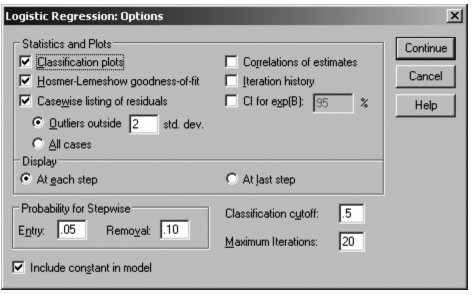
\includegraphics[scale=0.8]{images/Logistic10}\\
  \caption{Selected Options for Exercises}
\end{center}
\end{figure}

We are not using any categorical variables this time. If there are categorical variables, use the \textbf{\textit{categorical}} option. For most situations, choose the ‘indicator’ coding scheme (it is the
default).
\subsection{SPSS Outout  - Block 0: Beginning Block.}
Block 0 presents the results with only the constant included
before any coefficients (i.e. those relating to family size and mortgage) are entered into
the equation. Logistic regression compares this model with a model including all the
predictors (family size and mortgage) to determine whether the latter model is more
appropriate. The table suggests that if we knew nothing about our variables and guessed
that a person would not take the offer we would be correct 53.3\% of the time.
\begin{figure}[h!]
\begin{center}
  % Requires \usepackage{graphicx}
  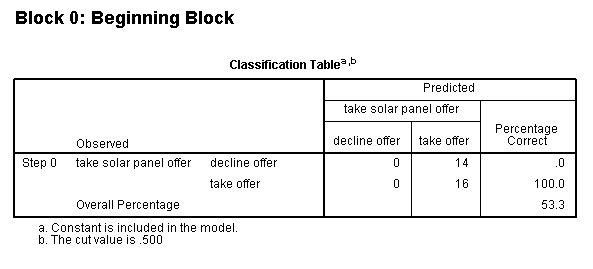
\includegraphics[scale=0.6]{images/Logistic3}\\
  \caption{Classification table}
\end{center}
\end{figure}
The variables not in the equation table tells us whether each IV improves the model. The answer is yes for both variables, with family size slightly better than mortgage size, as both are significant and if included would add to the predictive power of the model. If they had not been significant and able to contribute to the prediction,
then termination of the analysis would obviously occur at this point

\begin{figure}
\begin{center}
  % Requires \usepackage{graphicx}
  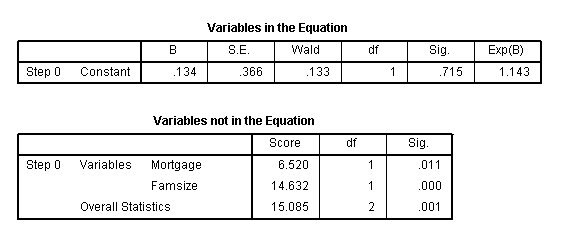
\includegraphics[scale=0.6]{images/Logistic4}\\
  \caption{Variables in / not in the equation}
\end{center}
\end{figure}
This presents the results when the predictors ‘family size’ and
‘mortgage’ are included. Later SPSS prints a classification table which shows how the
classification error rate has changed from the original 53.3%. By adding the variables
we can now predict with 90\% accuracy (see Classification Table later). The
model appears good, but we need to evaluate model fit and significance as well. SPSS will
offer you a variety of statistical tests for model fit and whether each of the independent
variables included make a significant contribution to the model.
\begin{figure}
\begin{center}
  % Requires \usepackage{graphicx}
  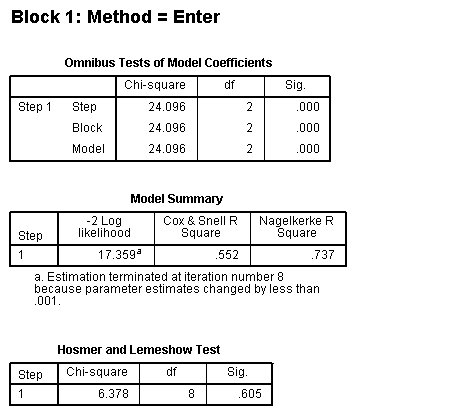
\includegraphics[scale=0.6]{images/Logistic5}\\
  \caption{Test Outcomes}
\end{center}
\end{figure}
\subsection{Omnibus Test for Model Coefficients}
The overall significance is tested using what SPSS calls the \textbf{\textit{Model Chi-square}}, which is derived from the likelihood of observing the actual data under the assumption that the model that has been fitted is accurate. There are two hypotheses to test in relation to the overall fit of the model:


 \begin{itemize}
 \item[$H_0$] The model is a good fitting model.
 \item[$H_1$] The model is not a good fitting model (i.e. the predictors have a significant effect).
 \end{itemize}
 In our case model chi square has 2 degrees of freedom, a value of 24.096 and a probability of $p < 0.000$.

Thus, the indication is that the model has a poor fit, with the model containing only the constant indicating that the predictors do have a significant effect and create essentially a different model. So we need to look closely at
the predictors and from later tables determine if one or both are significant predictors.

This table has 1 step. This is because we are entering both variables and at the same
time providing only one model to compare with the constant model. In stepwise logistic regression there are a number of steps listed in the table as each variable is added or
removed, creating different models. The step is a measure of the improvement in the
predictive power of the model since the previous step. ( I will revert to this next class).

%The likelihood function can be thought of as a measure of how well a candidate model fits the data (although that is a very simplistic definition). The AIC criterion is based on the Likelihood function.
%The likelihood function of a fitted model is commonly re-expressed as -2LL (i.e. The log of the likelihood times minus 2).

%The difference between –2LL for the best-fitting model and –2LL for the null hypothesis model (in which all the b values are set to zero in block 0) is distributed like
%chi squared, with degrees of freedom equal to the number of predictors; this difference
%is the Model chi square that SPSS refers to. Very conveniently, the difference between –2LL values for models with successive terms added also has a chi squared distribution,
%so when we use a stepwise procedure, we can use chi-squared tests to find out if adding
%one or more extra predictors significantly improves the fit of our model.


\subsection{Model Summary Table}


The likelihood function can be thought of as a measure of how well a candidate model fits the data (although that is a very simplistic definition). The AIC criterion is based on the Likelihood function.
The likelihood function of a fitted model is commonly re-expressed as -2LL (i.e. The log of the likelihood times minus 2). The –2LL value from the Model Summary table below is 17.359.

Although there is no close analogous statistic in logistic regression to
the coefficient of determination $R^2$ the Model Summary Table provides some approximations. Cox and Snell’s R-Square attempts to imitate multiple R-Square based on ‘likelihood’, but its maximum can be (and usually is) less than 1.0, making it difficult to interpret. Here it is indicating that 55.2\% of the variation in the DV is explained by the
logistic model. The Nagelkerke modification that does range from 0 to 1 is a more reliable
measure of the relationship. Nagelkerke’s $R^2$ will normally be higher than the Cox and Snell measure. Nagelkerke’s $R^2$ is part of SPSS output in the ‘Model Summary’ table and is the most-reported of the R-squared estimates. In our case it is 0.737, indicating a moderately strong relationship of 73.7\% between the predictors and the prediction.
\newpage
\subsection{Hosmer and Lemeshow  Statistic}
An alternative to model chi square is the Hosmer and Lemeshow test
which divides subjects into 10 ordered groups of subjects and then compares the number
actually in the each group (observed) to the number predicted by the logistic regression
model (predicted). The 10 ordered groups are created based on their estimated probability; those with estimated probability below .1 form one group, and so on, up to those with probability .9 to 1.0.

Each of these categories is further divided into two groups based on the actual observed outcome variable (success, failure). The expected frequencies for each of the cells are obtained from the model. A probability (p) value is
computed from the chi-square distribution with 8 degrees of freedom to test the fit of the logistic model.

If the H-L goodness-of-fit test statistic is greater than .05, as we want for well-fitting models, we fail to reject the null hypothesis that there is no difference between observed and model-predicted values, implying that the model’s estimates fit the data at an acceptable level. That is, well-fitting models show non-significance on the
H-L goodness-of-fit test. This desirable outcome of non-significance indicates that the
model prediction does not significantly differ from the observed.

The H-L statistic assumes sampling adequacy, with a rule of thumb being enough cases so that 95\% of cells (typically, 10 decile groups times 2 outcome categories = 20 cells) have an expected frequency $>$ 5. Our H-L statistic has a significance of .605 which means that it is not statistically significant and therefore our model is quite a
good fit.
\begin{figure}[h!]
\begin{center}
  % Requires \usepackage{graphicx}
  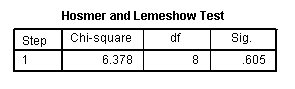
\includegraphics[scale=0.6]{images/Logistic7A}\\
  \caption{Hosmer and Lemeshow Statistic}
\end{center}
\end{figure}

\begin{figure}[h!]
\begin{center}
  % Requires \usepackage{graphicx}
  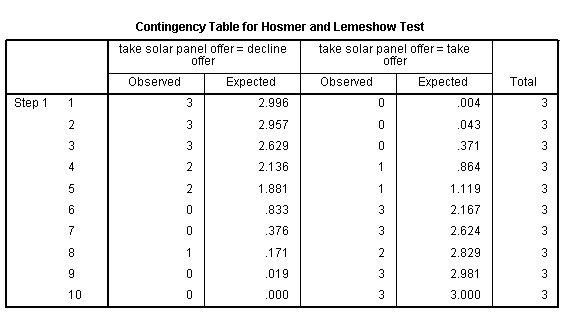
\includegraphics[scale=0.6]{images/Logistic6}\\
  \caption{Hosmer and Lemeshow Table}
\end{center}
\end{figure}
\newpage
\subsection{Classification Table}
Rather than using a goodness-of-fit statistic, we often want to look at the proportion of cases we have managed to classify correctly. For this we need to look at the classification table printed out by SPSS, which tells us how many of the cases where the observed values of the dependent variable were 1 or 0 respectively have
been correctly predicted.

In the Classification table, the columns are the two predicted values of the dependent, while the rows are the two observed (actual) values of the dependent. In a perfect model, all cases will be on the diagonal and the
overall percent correct will be 100\%. In this study, 87.5\% were correctly classified for the take offer group and 92.9\% for the decline offer group. Overall 90\% were correctly classified. This is a considerable improvement on the 53.3\% correct classification with the constant model so we know that the model with predictors is a significantly better mode.
\begin{figure}[h!]
\begin{center}
  % Requires \usepackage{graphicx}
  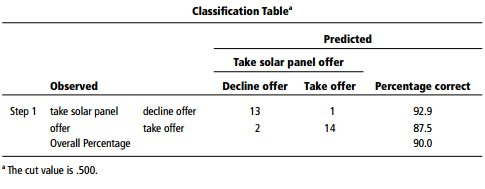
\includegraphics[scale=0.6]{images/Logistic7}\\
  \caption{Classification Table}
\end{center}
\end{figure}

\subsection{Variables in the Equation}
The Variables in the Equation table has several important elements. The Wald statistic and associated probabilities provide an index of the significance of each predictor in the equation.
The simplest way to assess Wald is to take the significance values and if less
than 0.05 reject the null hypothesis as the variable does make a significant contribution.
In this case, we note that family size contributed significantly to the prediction
(p = .013) but mortgage did not (p = .075). The researcher may well want to drop
independents from the model when their effect is not significant by the Wald statistic
(in this case mortgage).

\begin{figure}
\begin{center}
  % Requires \usepackage{graphicx}
  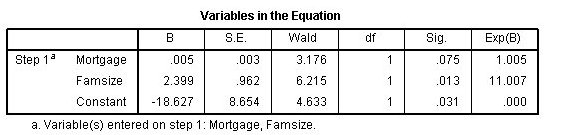
\includegraphics[scale=0.6]{images/Logistic8}\\
  \caption{Variables in the Equation}
\end{center}
\end{figure}

The \textbf{\textit{Exp(B)}} column in the table presents the extent to which raising the corresponding measure by one unit influences the odds ratio. We can interpret \textbf{\textit{Exp(B)}}) in
terms of the change in odds. If the value exceeds 1 then the odds of an outcome occurring increase; if the figure is less than 1, any increase in the predictor leads to a drop in
the odds of the outcome occurring. For example, the \textbf{\textit{Exp(B)}} value associated with
family size is 11.007. Hence when family size is raised by one unit (one person) the
odds ratio is 11 times as large and therefore householders are 11 more times likely to
belong to the take offer group.

The \textbf{\textit{B}} values are the logistic coefficients that can be used to create a predictive
equation (similar to the b values in linear regression) formula seen previously.
\begin{figure}
\begin{center}
  % Requires \usepackage{graphicx}
  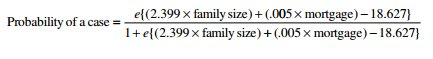
\includegraphics[scale=0.75]{images/Logistic11}\\
  \caption{Logistic Regression Equation}
\end{center}
\end{figure}

Here is an example of the use of the predictive equation for a new case. Imagine a
householder whose household size including themselves was seven and paying
a monthly mortgage of $2,500$ euros. Would they take up the offer, i.e. belong to category 1?
Substituting in we get:
\begin{figure}
\begin{center}
  % Requires \usepackage{graphicx}
  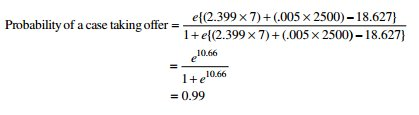
\includegraphics[scale=0.75]{images/Logistic12}\\
  \caption{Logistic Regression Equation : Example}
\end{center}
\end{figure}

Therefore, the probability that a householder with seven in the household and a mortgage of 2,500 p.m. will take up the offer is 99\%, or 99\% of such individuals will be
expected to take up the offer.
Note that, given the non-significance of the mortgage variable, you could be justified
in leaving it out of the equation. As you can imagine, multiplying a mortgage value by
B adds a negligible amount to the prediction as its B value is so small (.005).

\end{document}
